\section{Analysis}


For a better understanding of ICL-SC, 
we did comprehensive ablation studies and combined it with the traditional CL. The experiments in this section are done on dialogue summarization, which is representative due to the medium output length.




\subsection{Ablations on the Training Strategy}

%1. strategy: increase; decrease; random
To examine the design of decreasing the prefix for ICL-SC, we introduce the alternatives as follows:
\begin{itemize}
	\item \textbf{Decrease} refers to the Algorithm~\ref{alg:picl}. Taking $p_{start}=0.6$ and $s=0.3$ as an example, the prefix percentage $p$ varies as $0.6\rightarrow 0.3\rightarrow 0.0$ during training.
	\item \textbf{Increase} means that we gradually increase the length of prefix by increase $p$ following $0.0\rightarrow0.3\rightarrow0.6$.
	\item \textbf{Random} is that we randomly pick $p$ from the set $\{0.0, 0.3, 0.6\}$ in this example.
\end{itemize}


\begin{table}[h]
	\scriptsize
	\centering
	\begin{tabular}{cccccc}
		\hline
		{Strategy} & {R1} & {R2} & {RL} & {Met} & {BertS} \\
		\hline
		Decrease &\textbf{53.07} & \textbf{28.23} & \textbf{43.83} & \textbf{26.12} & \textbf{72.17}\\
		Increase & 51.43 & 27.35 & 42.97 & 24.32 & 71.25 \\
		Random & 51.80 & 27.69 & 43.27 & 24.59 & 71.51 \\
		\hline
	\end{tabular}
	\caption{Ablations on ICL strategies. The starting point and the stride are 0.6 and 0.3 respectively.}
	\label{tab:ablstrategy}
\end{table}

The results are shown in Table~\ref{tab:ablstrategy}, with Decrease ranking first and Increase ranking the worst.
Decrease significantly outperforms other ablations, showing that our sequence completion criterion of shrinking the prefix does work by means of learning from easy to hard.
%, instead of the implicit ``data augmentation'' which calculates different losses given the same sample during training.




\subsection{Parameter Search of the Starting Point and the Stride}
\label{sec:params}

To better understand how the ICL-SC manipulates the difficulty of samples during the training process, we further did experiments on different settings of two newly-introduced hyper-parameters $p_{start}$ and $s$. The results are in ~\figref{fig:stridestart}.

\begin{figure}[h]
	\centering
	\begin{minipage}[t]{0.5\linewidth}
		\centering
		\subfloat[Starting Point]{
			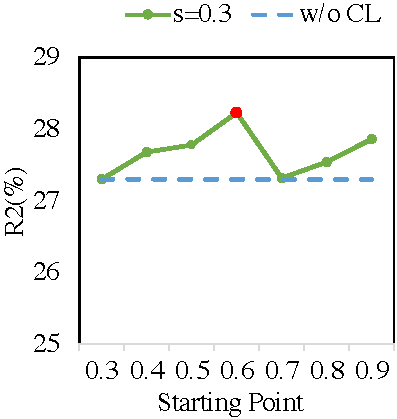
\includegraphics[scale=0.45]{start.pdf}
			%\caption{fig1}
		}%
	\end{minipage}%
	\begin{minipage}[t]{0.5\linewidth}
		\centering
		\subfloat[Stride]{
			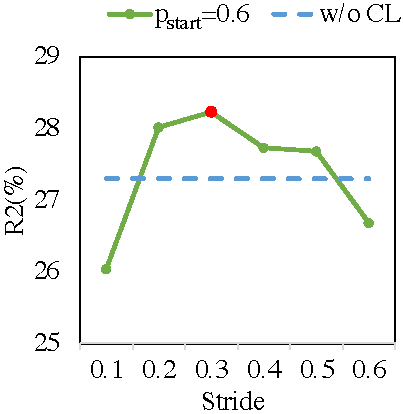
\includegraphics[scale=0.45]{stride.pdf}
			%\caption{fig2}
		}%
	\end{minipage}%
	\centering
	\caption{Parameter search of the starting point $p_{start}$ and the stride $s$. The ``w/o'' CL representing the BART baseline is drawn for comparison.} %Ablations on the starting point of ICL-SC with $s=0.3$ and ablations on the stride of ICL-SC with $p_{start}=0.6$. 
	\label{fig:stridestart}
\end{figure}


We can see that the performance drops with either a too large or too small $p_{start}$. The former one starts training with only predicting the last 1 or 2 tokens according to the average length of reference output shown in Table~\ref{tab:taskdata}. Most of the time, they are punctuation marks that do not carry any important semantic information, leading to a bad warm-up. The latter one requires the model to predict more than half of the output, which are too difficult as a beginning learning target. Besides, a larger $p_{start}$ which is divisible by $s$ is more competitive.
%All of the results still outperforms the original baseline.

The trend is the same for using different stride values. The performance drops with $s$ equaling 0.1 or 0.6. 
The smaller ones lead to too tiny changes, which not only excessively prolongs the required training time but also leads to server outfitting on the training set. The larger ones greatly enlarge the gap between training targets which degrades to 0.0 directly. It also harms the performances.

In a word, the training should start with a medium difficulty training objective and the gap between training objectives shouldn't be too large. Both parameters are closely related to the output length of different tasks. We suggest using ($p_{start}=0.6$, $s=0.3$) for NLG tasks with multi-sentence outputs, and ($p_{start}=0.5$, $s=0.5$) for NLG tasks with single-sentence outputs. All of our experiments are done based on this guideline. %More insights on the relation between the average output length and parameter settings are expected as future work.

%2. hyper-parameters of starting point: 0.6,0.7,0.8,0.9,  0.3,0.4,0.5

%\begin{table}[t]
%	\scriptsize
%	\centering
%	\begin{tabular}{ccccccc}
%		\hline
%		{Start} & {Stride}& {R1} & {R2} & {RL} & {Met} & {BertS} \\
%		\hline
%		0.9 &\multirow{7}{*}{0.3}& 52.97 & 27.86 & {43.72} & \textbf{26.23} & 71.89 \\
%		0.8 & &52.54 & 27.54 & 43.44 & 26.08 & 71.92 \\
%		0.7 & &52.46 & 27.32 & 43.32 & 25.26 & 71.32\\
%		0.6 & &\textbf{53.07} & \textbf{28.23} & \textbf{43.83} & 26.12 & \textbf{72.17}\\
%		0.5 & &52.37 & 27.78 & 43.54 & 25.31 & 71.74 \\
%		0.4 & &52.14 & 27.68 & 43.20 & 25.09 & 71.52 \\
%		0.3 & &51.46 & 27.30 & 42.74 & 24.37 & 71.15\\
%		\hline
%		\multirow{6}{*}{0.6}&0.1  & 50.75 & 26.04 & 41.86 & 24.06 & 70.81\\
%		&0.2 & 52.46 & 28.02 & 43.63 & 25.21 & 71.79\\
%		&0.3 & \textbf{53.07} & \textbf{28.23} & \textbf{43.83} & \textbf{26.12} & \textbf{72.17} \\
%		&0.4 & 51.90 & 27.73 & 43.09 & 25.11 & 71.53\\
%		&0.5 & 51.84 & 27.68 & 43.15 & 24.99 &71.73\\
%		&0.6 & 50.86 & 26.68 & 42.32 & 23.55 &70.76\\
%		\hline
%		w/o & w/o &51.88 & 27.30 & 42.77 & 24.75 & 71.38 \\
%		\hline
%	\end{tabular}
%	\caption{Ablations on the starting point of propotional ICL with the stride equaling 0.3 and ablations on the stride of propotional ICL with the starting point equaling 0.6. The last line with ``w/o'' representing the BART baseline without using the ICL strategy is listed for comparison.}
%	\label{tab:ablstart}
%\end{table}


\subsection{Combinations with the Traditional CL}


Since our ICL-SC is orthogonal to sample-wise CL and designing an appropriate sample-wise curriculum is not easy, we choose dialogue summarization as a representative task, design several traditional CL strategies empirically, and further apply our ICL-SC on top of them for comparisons.
$4$ different traditional CL strategies are as follows:
\begin{itemize}
	\item \textbf{Input length (InLen)} refers to the number of tokens in the input dialogue. The longer a dialogue is, the more complex a sample is.
	\item \textbf{Output length (OutLen)} is the number of tokens in a reference summary, which is also proportional to the difficulty of a sample.
	\item \textbf{Compression ratio (CompR)} equals the output length divided by the input length. More compressed training pairs are harder.% for models to learn from. %We generally agree that 
	\item \textbf{Abstractiveness (Abstr)} represents the percentage of novel words in the reference summary which are not in the dialogue. We measure it by Rouge-2 recall, which is inversely proportional to the difficulty level.
\end{itemize}

\begin{table}[th]
	\scriptsize
	\centering
	\begin{tabular}{lccccc}
		\hline
		{Method} & {R1} & {R2} & {RL} & {Met} & {BertS} \\
		\hline
		w/o CL & 51.88 & 27.30 & 42.77 & 24.75 & 71.38 \\
		ICL-SC & {\textbf{53.07}} & \textbf{28.23} & \textbf{43.83} & {\textbf{26.12}}& {\textbf{72.17}} \\
		\hline
		InLen & 52.19 & \textbf{27.73} & \textbf{43.50} & 25.57 & 71.73\\
		InLen+ & \textbf{52.56} & 27.60 & 43.43 & \textbf{25.77} & \textbf{71.92}\\
		\hline
		OutLen & 41.38 & 20.88 & 31.77 & \textbf{27.95} & 67.21\\
		OutLen+ &\textbf{43.96} & \textbf{22.14} & \textbf{33.05} & 26.39 & \textbf{67.64} \\
		\hline
		CompR & 39.68 & 19.28 & 34.73 & 14.41 & 65.96 \\
		CompR+ & \textbf{41.59} & \textbf{20.78} & \textbf{36.62} & \textbf{15.22} & \textbf{67.19}\\
		\hline
		Abstr & \textbf{44.61} & 20.10 & 36.93 & \textbf{17.34} & 68.29 \\
		Abstr+ & 44.41 & \textbf{20.64} & \textbf{37.29} & 17.25 & \textbf{68.33} \\
		\hline
	\end{tabular}
	\caption{Performaces with traditional CL strategies. ``+'' represents experiments further armed with ICL-SC.}
	\label{tab:traditional}
\end{table}
The results based on the ordered training samples according to these intuitive CL strategies are shown in Table~\ref{tab:traditional}. It shows that only InLen improves the vanilla model, but it still lags behind the pure ICL-SC. Other strategies failed mainly due to the low data quality at the beginning or the end of training. 
Taking Abstr as an example, samples with the highest 
Rouge-2 recall are gathered at the beginning where 
their inputs and outputs are almost the same. 
This leads to a bad initialization for models learning 
the summarization ability. 

Besides, some strategies 
are incompatible, such as OutLen and CompR. Samples with the shortest output length are always too compressed. Therefore, developing a comprehensive score for a better ranking is difficult. It should be also noticed that most of these strategies are designed for summarization, which are not suitable for generalization.

In a word, it's hard to develop a 
comprehensive strategy for one task or a unified strategy for different NLG tasks with traditional CL. 
%Our ICL-SC can be easily combined with these CL strategies. %by training with ordered training samples instead of random sampling. 
ICL-SC not only outperforms these CL strategies, but also improves them when easily combined. 

\label{sec:tracl}


%\subsection{Performance on Variable Lengths}

%\begin{table}
%	\small
%	\centering
%	\begin{tabular}{lcccccc}
%	\hline
%	Dataset &  Avg & Std & \#1 & \#2 & \#3 & \#4 \\
%	\hline
%	DREAM & 5.59 & 2.61 & 483 & 653 & 468 & 483 \\
%	\hline
%	SAMSum & 24.99 & 13.06 & 227 & 260 & 170 & 162 \\	
%	\hline
%	\multirow{2}{*}{Shakespeare} & 12.24 & 9.27 & 423 & 288 & 290 & 461 \\
%	& 11.02 & 7.10 & 423 & 328 & 264 & 447 \\
%	\hline
%	SQuAD1.1 & 13.09 & 4.27 & 2330 & 4755 & 3041 & 1751 \\
%	\hline
%	CNNDM & \\
%	\hline
%	\end{tabular}
%	\caption{Statistics on variable output length. Avg and Std refer to the average and the standard deviation of the output length. \#1 to \#4 represent the number of samples belonging to different test buckets divided by the output length in ascending order.
%	Shakespeare contains two rows as its output can be in both styles.}
%	\label{tab:ablength}
%\end{table}

%\begin{figure*}[th]
%	\centering

%		\begin{minipage}[t]{0.5\linewidth}
%			\centering
%				\subfloat[Dialogue Summarization]{
%			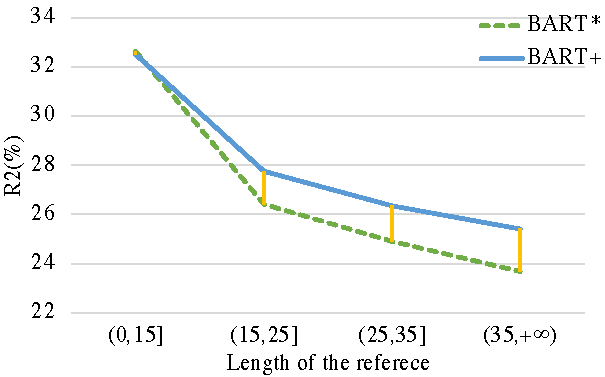
\includegraphics[scale=0.65]{length-ds.pdf}
%\caption{fig1}
%				}%
%		\end{minipage}%
%		\begin{minipage}[t]{0.5\linewidth}
%			\centering
%				\subfloat[Reading Comprehension]{
%			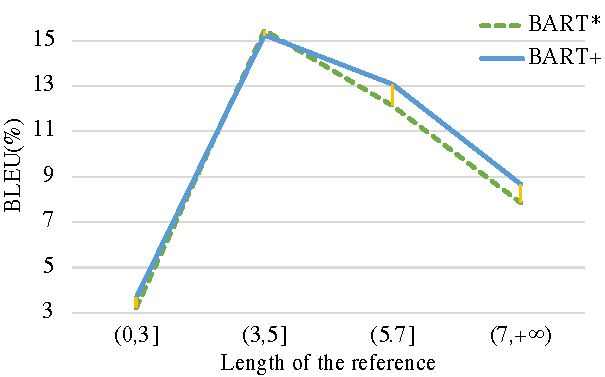
\includegraphics[scale=0.65]{length-rc.pdf}
%\caption{fig2}
%				}%
%		\end{minipage}%

%		\begin{minipage}[t]{0.5\linewidth}
%			\centering
%			\subfloat[Style Transfer]{
%				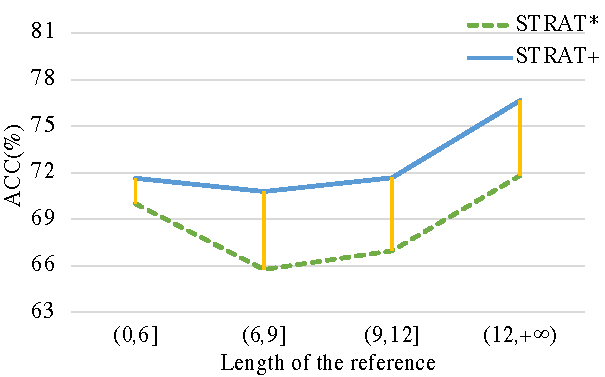
\includegraphics[scale=0.65]{length-st.pdf}
%\caption{fig2}
%			}%
%		\end{minipage}%
%		\begin{minipage}[t]{0.5\linewidth}
%			\centering
%			\subfloat[Question Generation]{
%				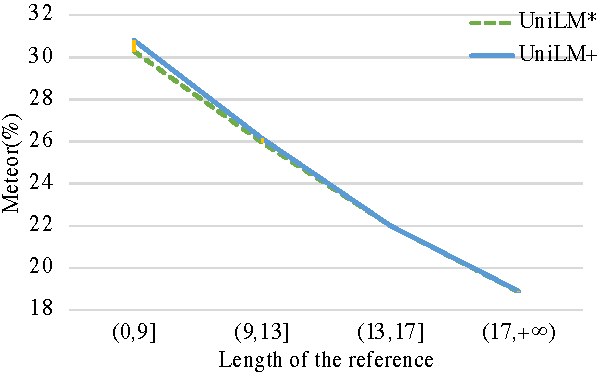
\includegraphics[scale=0.65]{length-qg.pdf}
%\caption{fig2}
%			}%
%		\end{minipage}
%	\centering
%	\caption{Comparisons on variable lengths. \KZ{The label should read
%Length of the ``reference'' text.}}
%	\label{fig:ablength}
%\end{figure*}





